% meta.concepts: 2D moment
% meta.tags: realistic
% acknowledge: Peter Seiler & Luke Melander graciously shared Spring 2019 course material
% source: 2019 P. Seiler AEM2011 HW 3 (variations made)


% Weight used: 38.12 kg.  Not shown to avoid confusion for students.
\noindent A tightrope walker is attempting a walk across a 50 meter span 20 meters above the ground. When
he is 20\% across the span, the rope is deflected such that he is 17 meters above the ground. 
At this point the tension in the cable behind and ahead of the walker is 1,041.1 N and 1,000.0 N, respectively.
\newline
\noindent Find the moments caused by the cable tension about points A and B (where the support posts meet the ground).


\begin{figure}[ht!]
  \centering
  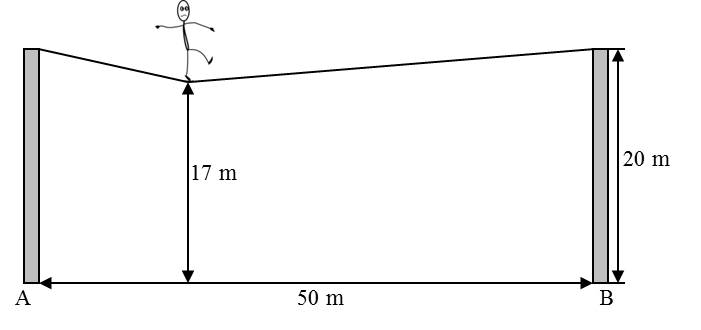
\includegraphics[height=1.8in]{fig.png}
\end{figure}

